%%%%%%%%%%%%%%%%%%%%%%%%%%%%%%%%%%%%%%%%%%%%%%%%%%%%%%%%%%%%%%%%%%%%%%
% How to use writeLaTeX: 
%
% You edit the source code here on the left, and the preview on the
% right shows you the result within a few seconds.
%
% Bookmark this page and share the URL with your co-authors. They can
% edit at the same time!
%
% You can upload figures, bibliographies, custom classes and
% styles using the files menu.
%
%%%%%%%%%%%%%%%%%%%%%%%%%%%%%%%%%%%%%%%%%%%%%%%%%%%%%%%%%%%%%%%%%%%%%%

\documentclass[12pt]{article}

\usepackage{sbc-template}
\usepackage{graphicx,url}
\usepackage{float}
\usepackage{array}
\usepackage{tabularx}
\usepackage{makecell}

\usepackage{tcolorbox}
\usepackage{minted}

\usepackage[utf8]{inputenc}  

\tcbset{
  codeSnippetStyle/.style={
    colback=gray!10, % cor de fundo mais clara
    colframe=gray!30!, % cor da borda
    title=#1, % título da caixa
    coltitle=black, % cor do título
    boxrule=0.2mm, % espessura da borda
    arc=3mm, % arredondamento dos cantos
    width=\textwidth, % largura da caixa
    boxsep=7pt
  }
}

\newcolumntype{Y}{>{\centering\arraybackslash}X}

\sloppy

\title{Análise da Aderência às Boas Práticas de Desenvolvimento em Projetos Open Source Flutter: Primeiros Insights}
\author{Anonymous\inst{1}}

\address{Anonymous \email{\{anonymous\}@anonymous}}

\begin{document} 

\maketitle

\begin{abstract}
This research investigates adherence to development practices in open-source Flutter projects, focusing on code quality and maintainability. We analyzed 45 projects using SonarQube to identify Best Practice Violations (BPVs). A total of 10,120 BPVs were found, distributed across three severities: 5,149 minor, 4,273 major, and 698 critical violations. We calculated the Pearson correlation coefficient to confirm the relationship between BPVs and non-commenting lines of code (NCLOC) and between BPVs and cyclomatic complexity. We observed a strong correlation (0.8978) between BPVs and NCLOC, and a moderate correlation (0.4509) between BPVs and complexity. These results indicate, for the studied context, that the best practices recommended by the Dart main team are not being followed and that there is a need for improvement in the quality of Flutter application code..
\end{abstract}
     
\begin{resumo} 
Esta pesquisa investiga a adesão às melhores práticas de desenvolvimento em projetos open-source Flutter, focando na qualidade e manutenibilidade do código. Foram analisados 45 projetos utilizando o SonarQube para identificar Violações de Boas Práticas (VBPs). Foram encontradas 10.120 VBPs, distribuídas em três severidades: 5.149 Leves, 4.273 Graves e 698 Críticas. O coeficiente de correlação de Pearson foi calculado para confirmar a relação entre VBPs e linhas de código (LCNC) e entre VBPs e complexidade ciclomática. Observou-se uma correlação forte (0,8978) entre VBPs e LCNC, e uma correlação moderada (0,4509) entre VBPs e complexidade. Esses resultados indicam, para o contexto estudado, que as boas práticas recomendadas pela equipe do Dart não estão sendo seguidas e que existe uma necessidade de melhoria na qualidade do código de aplicações Flutter.
\end{resumo}

\section{Introdução}
A evolução tecnológica acelerada tem modificado substancialmente a interação com o mundo digital, com os dispositivos móveis emergindo como agentes principais dessa transformação. No Brasil, a média de 1,2 smartphones por habitante causa uma demanda crescente por serviços digitais e aplicativos móveis. Em 2022, por exemplo, os investimentos em tecnologia da informação (TI) corresponderam a 9\% do faturamento das empresas, refletindo também em um aumento significativo no desenvolvimento de aplicativos móveis \cite{FGVcia2023}.

Lançado pelo Google em 2017, o Flutter é um \textit{framework} de código aberto que se tornou popular por permitir que desenvolvedores criem aplicativos que funcionam em múltiplos sistemas operacionais, como Android e iOS, com mínimas alterações no código-fonte \cite{flutter}. Utilizando a linguagem de programação Dart, também desenvolvida pelo Google, o Flutter facilita a escrita de código e a manutenção a longo prazo. Além disso, se destaca pelo motor gráfico próprio, que oferece consistência e desempenho em diferentes plataformas, e pelo ecossistema de pacotes e \textit{plugins} disponíveis no Pub, o gerenciador de pacotes do Dart.

Para garantir que os aplicativos desenvolvidos com Flutter mantenham sua robustez e sejam facilmente mantidos ao longo do tempo, a equipe principal do Dart elaborou um conjunto de melhores práticas de desenvolvimento~\cite{dartBestPractices}. Inspirados em princípios do \textit{clean code} \cite{fowler1999refactoring}, as recomendações tem foco na legibilidade, consistência, concisão e eficiência do código \cite{dartBestPractices}. Essas diretrizes estão descritas no guia ``Effective Dart'', que inclui recomendações sobre estilo, documentação e práticas específicas para desenvolvimento em Dart e Flutter \cite{dartBestPractices}.

Neste contexto, este estudo investiga a adesão a essas melhores práticas de programação em projetos open source desenvolvidos com Flutter. Utilizou-se o conceito de Violações de Boas Práticas (VBPs), que são definidas como desvios das diretrizes estabelecidas pela equipe principal do Dart para garantir a escrita de código claro, eficiente e de fácil manutenção. A pesquisa visa responder as seguintes questões de pesquisa:
\begin{itemize}    
\item QP1- Qual a prevalência de VBPs nos projetos open source estudados?
\item QP2- Quais tipos de práticas são mais frequentemente violadas?
\end{itemize}

\section{Metodologia}

A metodologia adotada foi estruturada em quatro etapas principais: seleção de projetos, configuração das ferramentas de análise, coleta de dados e avaliação dos resultados. Além das VBPs, também foi analisada a complexidade do código dos projetos, medida por métricas como a complexidade ciclomática e número de linhas de código não comentadas (LCNC) \cite{mccabe1976complexity}.

\subsection{Seleção de Projetos}
A seleção dos projetos seguiu diretrizes propostas em \cite{baltes2022sampling}. Inicialmente, foram considerados os projetos open source Flutter recomendados pela comunidade e disponíveis no repositório \textit{Open-Source Flutter Apps}\footnote{Tortuvshin Bayarsaikhan. Open-Source Flutter Apps. 2023. Disponível em: \url{https://github.com/tortuvshin/open-source-flutter-apps}. Acessado em: 08 de julho de 2024}, que contava com 152 projetos em 15 de maio de 2024. Os projetos do repositório foram filtrados seguindo critérios criados a partir das recomendações do estudo \cite{kalliamvakou2016depth}:
\begin{enumerate}
    \item Projetos com no mínimo 30 commits, garantindo projetos com um histórico consistente de atividade.
    \item Último commit feito nos últimos 3 anos, assegurando atividade recente.
    \item Mínimo de 30 estrelas no GitHub, indicando relevância na comunidade.
\end{enumerate}

Dos 152 projetos, 50 preencheram os três critérios. Durante a fase de análise, mais 5 projetos foram excluídos devido a problemas técnicos (e.g.,incompatibilidades de versões de dependências e bibliotecas; uso de bibliotecas descontinuadas).


\subsection{Procedimento e Análise dos Resultados}
\textit{SonarQube}\footnote{\url{https://docs.sonarsource.com/sonarqube/}} foi usado para identificar VBPs, sendo ele uma plataforma reconhecida por sua capacidade de análise estática de código \cite{marcilio2019static}. Para análise, o \textit{SonnarScanner} foi configurado de forma específica para cada projeto e um \textit{plugin} para análise de Dart e Flutter\footnote{\url{https://github.com/insideapp-oss/sonar-flutter}} foi usado para coletar métricas como número de VBPs, severidade e complexidade ciclomática. Os seguintes passos foram seguidos:
\begin{enumerate}
    \item Configuração do ambiente Docker e instalação do SonarQube.
    \item Download e instalação do plugin para análise de Dart e Flutter.
    \item Configuração e execução do SonarScanner nos projetos selecionados.
\end{enumerate}
 
Os dados foram coletados através da API do SonarQube e armazenados em formato JSON. Scripts em Python foram usados para automatizar a coleta, tratamento e análise dos dados, garantindo consistência e precisão nos resultados. 

Os resultados foram analisados para identificar a prevalência e severidade das VBPs. Calculou-se também o coeficiente de correlação de Pearson para avaliar a relação entre VBPs e Linhas de Código Não Comentadas (LCNC) e entre VBPs e complexidade ciclomática. O dataset completo criado a partir desta pesquisa, contendo todas as VBPs encontradas e informações úteis sobre os projetos selecionados, está disponível online\footnote{\url{https://anonymous.4open.science/r/flutter-open-source-practices-analysis-F1F7/json-files/fetched_issues_data.json}}.

\section{Resultados}
\subsection{QP1- Qual a prevalência de VBPs nos projetos open source estudados?}
A análise dos 45 projetos open source desenvolvidos com Flutter revelou 10.120 VBPs. Estas foram distribuídas em três níveis de severidade: 5.149 menores, 4.273 maiores e 698 críticas, avaliando a adesão às melhores práticas de desenvolvimento. Em média, os projetos apresentaram 3,88 VBPs por arquivo, com um desvio padrão de 4,25, indicando uma variação significativa na aderência às boas práticas de desenvolvimento entre os projetos.

As correlações de Pearson calculadas estão na Figura~\ref{fig:vbps_vs_lcnc_and_vbps_vs_complexity}. Pode-se observar uma correlação forte (\textit{r} = 0,8978) entre VBPs e LCNC, indicando que mais linhas de código estão associadas a mais VBPs. Adicionalmente, a Figura~\ref{fig:vbps_vs_lcnc_and_vbps_vs_complexity} mostra uma correlação moderada (\textit{r} = 0,4509) entre VBPs e complexidade ciclomática, sugerindo que projetos com maior complexidade ciclomática tendem a ter mais VBPs.

\begin{figure}[H]
\centering
\includegraphics[width=0.45\textwidth]{images/correlação_entre_vbps_e_lcnc.png}
\includegraphics[width=0.45\textwidth]{images/correlação_entre_vbps_e_complexidade_ciclomática.png}
\caption{Correlação entre VBPs e LCNC (esquerda) e entre VBPs e Complexidade Ciclomática (direita)}
\label{fig:vbps_vs_lcnc_and_vbps_vs_complexity}
\end{figure}

\subsection{QP2- Quais tipos de práticas são mais frequentemente violadas?}
A Figura~\ref{fig:rule_distribution} mostra a distribuição das cinco regras de boas práticas mais frequentemente violadas nos projetos analisados. A VBP mais frequente foi a EC (\textit{Exhaustive Cases}), com um total de 1544 violações. Esta regra verifica se todas as possibilidades em uma enumeração são cobertas, garantindo que o código seja robusto e não falhe ao encontrar casos inesperados. A alta frequência de violações desta regra indica que os desenvolvedores muitas vezes deixam de tratar todos os casos possíveis em enumerações, o que pode levar a erros em tempo de execução e a um código menos confiável.

\begin{figure}[H]
\centering
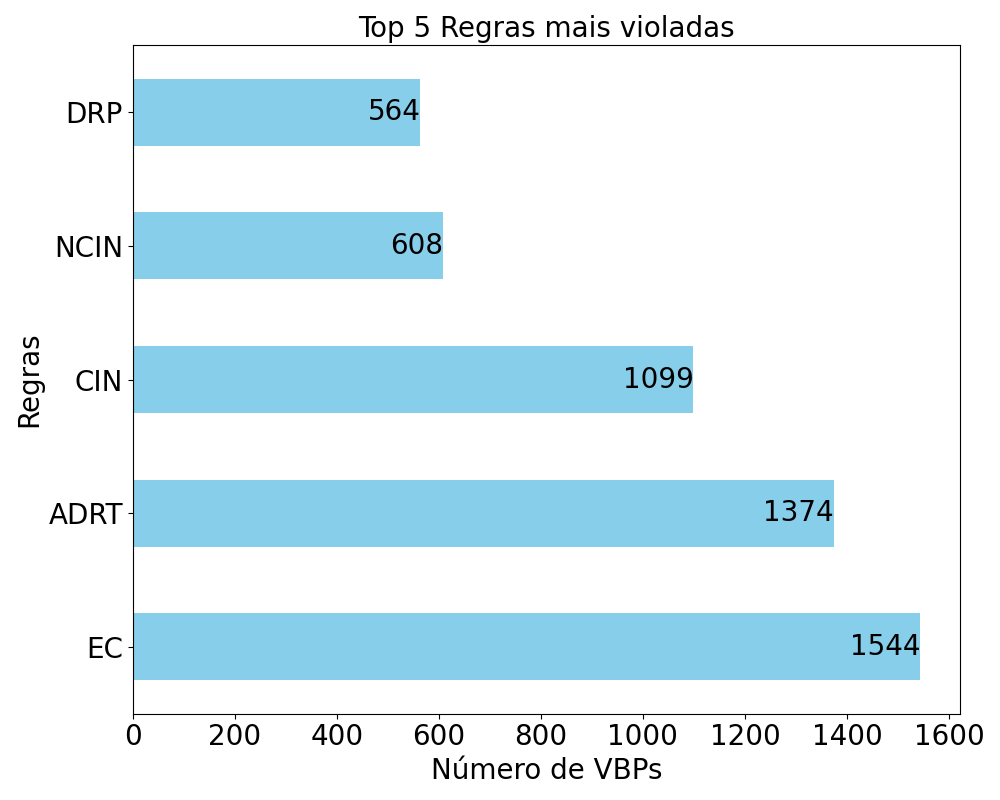
\includegraphics[width=.5\textwidth]{images/rule_distribution.png}
\caption{Distribuição das regras mais violadas}
\label{fig:rule_distribution}
\end{figure}

As siglas usadas no gráfico representam: \textbf{EC}: \textit{Exhaustive Cases}, verifica a cobertura completa de todos os casos possíveis de uma variável de enumeração em um \texttt{switch}; \textbf{ADRT}: \textit{Always Declare Return Types}, garante que todas as funções tenham tipos de retorno declarados; \textbf{CIN}: \textit{Constant Identifier Names}, verifica se os nomes das constantes estão em conformidade com as convenções de nomenclatura; \textbf{NCIN}: \textit{Non Constant Identifier Names}, verifica se os nomes dos identificadores não constantes estão em conformidade com as convenções de nomenclatura; \textbf{DRP}: \textit{Depend on Referenced Packages}, garante que as dependências declaradas estejam sendo utilizadas.

\subsection{Exemplo de Violação Crítica: Always Declare Return Types (ADRT)}
Entre as regras mais frequentemente violadas, a prática de declarar explicitamente os tipos de retorno de métodos (\textbf{ADRT}) se destaca por sua importância na manutenção e compreensão do código. No exemplo abaixo, retirado do repositório \textit{gsy\_github\_app\_flutter} \footnote{CarGuo. gsy\_github\_app\_flutter. Disponível em: \url{https://github.com/CarGuo/gsy\_github_app\_flutter/blob/3b7d9d2618305c8cab036bd11e5e6f9680ab6b00/lib/page/my\_page.dart#L41}. Acessado em: 10 de julho de 2024}, o método \texttt{getUserType}  não possui um tipo de retorno declarado, o que pode levar a problemas de manutenção e compreensão do código:

\begin{tcolorbox}[codeSnippetStyle={gsy\_github\_app\_flutter/lib/page/my\_page.dart}]
\begin{minted}[breaklines, fontsize=\footnotesize]{dart}
getUserType() {
  if (_getStore()?.state.userInfo == null) {
    return null;
  }
  return _getStore()?.state.userInfo?.type;
}
\end{minted}
\end{tcolorbox}

\section{Considerações Finais}
\subsection{Resultados Encontrados}
Esta pesquisa analisou 45 projetos open-source Flutter para identificar Violações de Boas Práticas (VBPs), encontrando mais de 10.000 violações distribuídas entre diferentes severidades. Esses resultados destacam áreas específicas onde melhorias podem ser feitas para aderir melhor às práticas recomendadas e melhorar a qualidade e manutenibilidade do código em projetos Flutter. Os resultados desta pesquisa mostram uma forte correlação entre o número de VBPs e as linhas de código não comentadas (LCNC), indicando que projetos maiores tendem a apresentar mais violações. Também foi observada uma correlação moderada entre VBPs e complexidade ciclomática, sugerindo que a complexidade do código influencia a qualidade do software.

As regras mais violadas, como Exhaustive Cases e Always Declare Return Types, indicam áreas onde os desenvolvedores devem concentrar esforços para melhorar a qualidade do código.
Para reduzir tais violações, uma abordagem eficaz é fomentar o uso de ferramentas de análise estática e verificação de código, como SonarQube e Dart Analyzer, durante o desenvolvimento.  Essas ferramentas podem identificar violações de boas práticas em tempo real, permitindo correções antes que se tornem significativas. A integração dessas ferramentas no processo de desenvolvimento contínuo pode ajudar a manter a qualidade do código, reduzir a complexidade ciclomática e evitar a duplicação de código \cite{kalagara2023measuring}.

\subsection{Trabalhos Futuros}
Para futuros trabalhos, espera-se realizar uma análise mais detalhada das causas das violações de boas práticas e uma investigação de processos automatizadas para auxiliar os desenvolvedores a aderirem a essas práticas. Outra possibilidade é expandir o conjunto de dados para incluir mais projetos e explorar a eficácia de diferentes ferramentas e metodologias de análise de código.

\bibliographystyle{sbc}
\bibliography{sbc-template}

\end{document}
